\documentclass[10pt]{article}
\usepackage[paperwidth=39cm, paperheight=39cm, margin=1cm]{geometry}
% Usuń numerację stron.
\pagestyle{empty}

\usepackage{tikz}
% Import do ustalania końcówek strzałek.
\usetikzlibrary{arrows.meta}

% Zmniejsz interlinię.
\linespread{0.9}

% Importy do białych konturów napisów.
\usepackage[T1]{fontenc}
\usepackage{pslatex}
\usepackage{contour}
\usepackage{color}
\contourlength{1pt} % Grubość konturu
\contournumber{50}  % Liczba powtórzeń

% Ustaw czcionkę bezszeryfową.
\renewcommand{\familydefault}{\sfdefault}

\begin{document}
\begin{figure}[p]
\centering
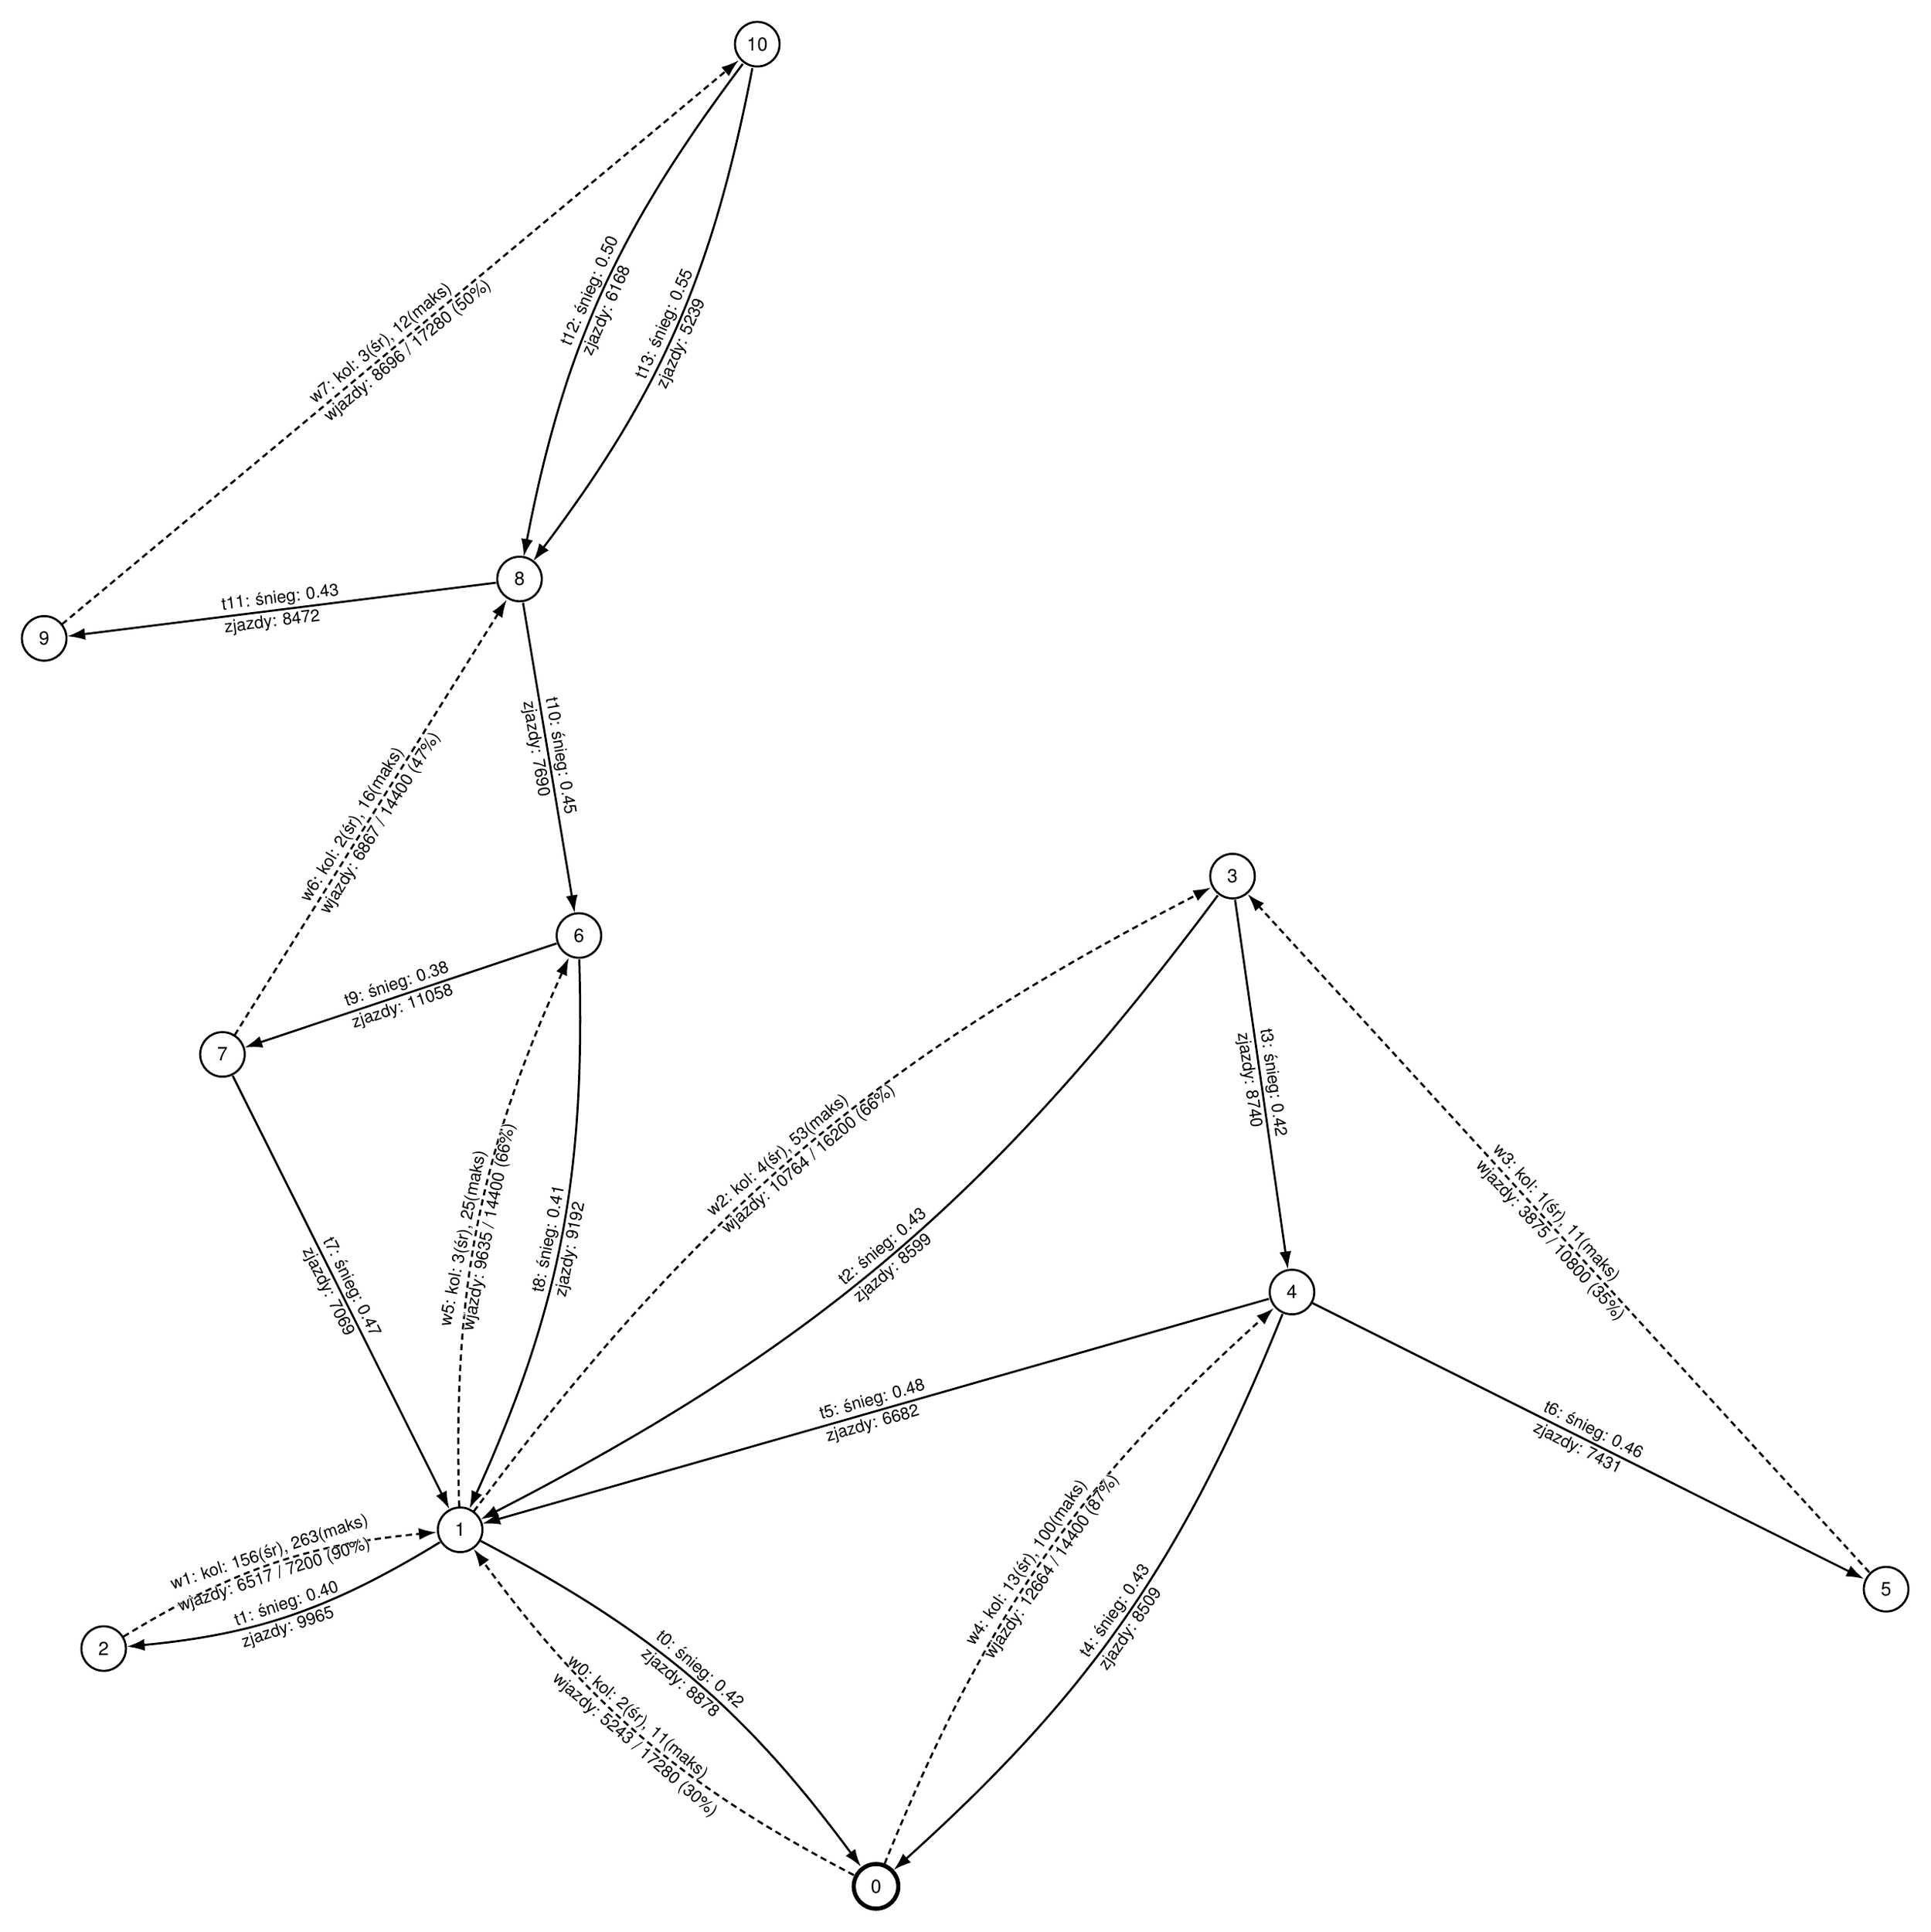
\begin{tikzpicture}[scale=100]
    \tikzset{
        % Style węzłów i krawędzi.
        wezel grafu/.style={circle,draw,minimum size=0.75cm,inner sep=0,line width=0.35mm},
        krawedz grafu/.style={-{Latex[length=3mm, width=2mm]},sloped,centered,line width=0.35mm,font=\small}
    }
    % Węzły:
    \node[wezel grafu,line width=0.7mm] (0) at (16/100, 2/100) {0};
    \node[wezel grafu] (1) at (9/100, 8/100) {1};
    \node[wezel grafu] (2) at (3/100, 6/100) {2};
    \node[wezel grafu] (3) at (22/100, 19/100) {3};
    \node[wezel grafu] (4) at (23/100, 12/100) {4};
    \node[wezel grafu] (5) at (33/100, 7/100) {5};
    \node[wezel grafu] (6) at (11/100, 18/100) {6};
    \node[wezel grafu] (7) at (5/100, 16/100) {7};
    \node[wezel grafu] (8) at (10/100, 24/100) {8};
    \node[wezel grafu] (9) at (2/100, 23/100) {9};
    \node[wezel grafu] (10) at (14/100, 33/100) {10};
    % Krawedzie:
    \path[draw]
    (0) edge[krawedz grafu, bend left=13, densely dashed] node {
        \begin{tabular}{l}
            \contour{white}{w0: kol: 2(śr), 11(maks)} \\
            \contour{white}{wjazdy: 5243 / 17280 (30\%)}
        \end{tabular}
    } (1)
    (1) edge[krawedz grafu, bend left=13] node {
        \begin{tabular}{l}
            \contour{white}{t0: śnieg: 0.42} \\
            \contour{white}{zjazdy: 8878}
        \end{tabular}
    } (0)
    (0) edge[krawedz grafu, bend left=13, densely dashed] node {
        \begin{tabular}{l}
            \contour{white}{w4: kol: 13(śr), 100(maks)} \\
            \contour{white}{wjazdy: 12664 / 14400 (87\%)}
        \end{tabular}
    } (4)
    (4) edge[krawedz grafu, bend left=13] node {
        \begin{tabular}{l}
            \contour{white}{t4: śnieg: 0.43} \\
            \contour{white}{zjazdy: 8509}
        \end{tabular}
    } (0)
    (1) edge[krawedz grafu, bend left=13] node {
        \begin{tabular}{l}
            \contour{white}{t1: śnieg: 0.40} \\
            \contour{white}{zjazdy: 9965}
        \end{tabular}
    } (2)
    (2) edge[krawedz grafu, bend left=13, densely dashed] node {
        \begin{tabular}{l}
            \contour{white}{w1: kol: 156(śr), 263(maks)} \\
            \contour{white}{wjazdy: 6517 / 7200 (90\%)}
        \end{tabular}
    } (1)
    (1) edge[krawedz grafu, bend left=13, densely dashed] node {
        \begin{tabular}{l}
            \contour{white}{w2: kol: 4(śr), 53(maks)} \\
            \contour{white}{wjazdy: 10764 / 16200 (66\%)}
        \end{tabular}
    } (3)
    (3) edge[krawedz grafu, bend left=13] node {
        \begin{tabular}{l}
            \contour{white}{t2: śnieg: 0.43} \\
            \contour{white}{zjazdy: 8599}
        \end{tabular}
    } (1)
    (4) edge[krawedz grafu] node {
        \begin{tabular}{l}
            \contour{white}{t5: śnieg: 0.48} \\
            \contour{white}{zjazdy: 6682}
        \end{tabular}
    } (1)
    (1) edge[krawedz grafu, bend left=13, densely dashed] node {
        \begin{tabular}{l}
            \contour{white}{w5: kol: 3(śr), 25(maks)} \\
            \contour{white}{wjazdy: 9635 / 14400 (66\%)}
        \end{tabular}
    } (6)
    (6) edge[krawedz grafu, bend left=13] node {
        \begin{tabular}{l}
            \contour{white}{t8: śnieg: 0.41} \\
            \contour{white}{zjazdy: 9192}
        \end{tabular}
    } (1)
    (7) edge[krawedz grafu] node {
        \begin{tabular}{l}
            \contour{white}{t7: śnieg: 0.47} \\
            \contour{white}{zjazdy: 7069}
        \end{tabular}
    } (1)
    (3) edge[krawedz grafu] node {
        \begin{tabular}{l}
            \contour{white}{t3: śnieg: 0.42} \\
            \contour{white}{zjazdy: 8740}
        \end{tabular}
    } (4)
    (5) edge[krawedz grafu, densely dashed] node {
        \begin{tabular}{l}
            \contour{white}{w3: kol: 1(śr), 11(maks)} \\
            \contour{white}{wjazdy: 3875 / 10800 (35\%)}
        \end{tabular}
    } (3)
    (4) edge[krawedz grafu] node {
        \begin{tabular}{l}
            \contour{white}{t6: śnieg: 0.46} \\
            \contour{white}{zjazdy: 7431}
        \end{tabular}
    } (5)
    (6) edge[krawedz grafu] node {
        \begin{tabular}{l}
            \contour{white}{t9: śnieg: 0.38} \\
            \contour{white}{zjazdy: 11058}
        \end{tabular}
    } (7)
    (8) edge[krawedz grafu] node {
        \begin{tabular}{l}
            \contour{white}{t10: śnieg: 0.45} \\
            \contour{white}{zjazdy: 7690}
        \end{tabular}
    } (6)
    (7) edge[krawedz grafu, densely dashed] node {
        \begin{tabular}{l}
            \contour{white}{w6: kol: 2(śr), 16(maks)} \\
            \contour{white}{wjazdy: 6867 / 14400 (47\%)}
        \end{tabular}
    } (8)
    (8) edge[krawedz grafu] node {
        \begin{tabular}{l}
            \contour{white}{t11: śnieg: 0.43} \\
            \contour{white}{zjazdy: 8472}
        \end{tabular}
    } (9)
    (10) edge[krawedz grafu, bend left=-13] node {
        \begin{tabular}{l}
            \contour{white}{t12: śnieg: 0.50} \\
            \contour{white}{zjazdy: 6168}
        \end{tabular}
    } (8)
    (10) edge[krawedz grafu, bend left=13] node {
        \begin{tabular}{l}
            \contour{white}{t13: śnieg: 0.55} \\
            \contour{white}{zjazdy: 5239}
        \end{tabular}
    } (8)
    (9) edge[krawedz grafu, densely dashed] node {
        \begin{tabular}{l}
            \contour{white}{w7: kol: 3(śr), 12(maks)} \\
            \contour{white}{wjazdy: 8696 / 17280 (50\%)}
        \end{tabular}
    } (10)
    ;
\end{tikzpicture}

\end{figure}
\end{document}
